\chapter{\label{ch:methodology} Methodology}
This chapter details the design and implementation of a mobile robotic system using augmented reality (AR), fiducial markers, and remote monitoring to improve human-robot interaction (HRI). It builds on existing research in computer vision-based navigation, AR for HRI, and internet-controlled mobile robots. Design decisions are justified with related literature and practical system requirements.

\section{\label{sec:overview} Overview}
The high-level diagram illustrates the mobile robot project's architecture, showcasing key components: Raspberry Pi (central processor), camera module, motor control system, fiducial markers, and web-based control interface. The data flow begins with the camera capturing video, which the Raspberry Pi processes for marker detection and navigation. Simultaneously, the web interface sends commands to the Raspberry Pi, which also streams video back to the user.

\begin{figure}[H]
	\centering
	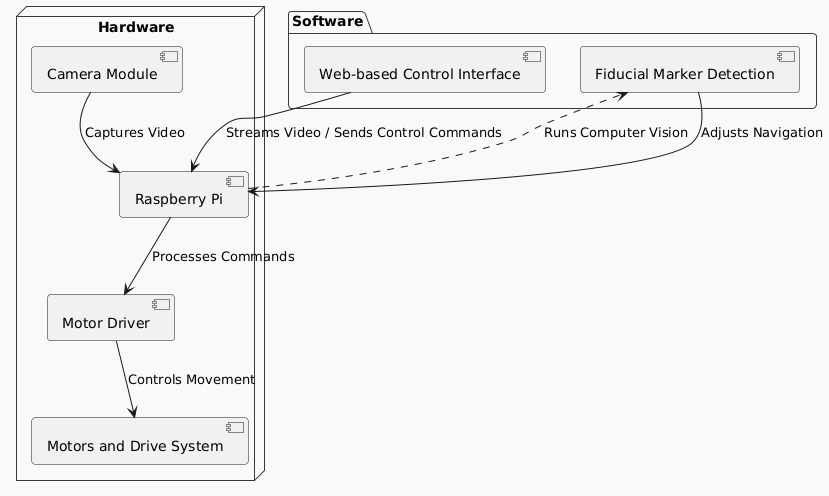
\includegraphics[width=0.8\textwidth]{ch3/figs/diagram.png}
	\caption{High Level Diagram of how the project will run}
	\label{fig:high_level_diagram}
\end{figure}

The methodology centers on the development of a mobile robot system capable of navigation, interaction, and real-time feedback, using AR markers and remote control via a Raspberry Pi board. Inspired by the works of La Delfa et al. \cite{delfa2015}, Jacobsen et al. \cite{jacobsen2018}, and Vanitha et al. \cite{vanitha2016}, this project seeks to incorporate advances in fiducial marker systems and AR interfaces to improve the efficiency and user engagement in controlling mobile robots.

\section{\label{sec:subsystems} Subsystems Overview}
This section delves into the various subsystems that form the mobile robot project, discussing their functions, components, and how they contribute to the overall project architecture.

\subsection{\label{subsec:camera} Camera Module}
The camera module is responsible for capturing real-time video, which is then sent to the Raspberry Pi for processing. The camera is positioned in such a way that it can capture the environment around the robot, ensuring that fiducial markers and obstacles are visible. This visual data is crucial for navigation and interaction as it enables the system to detect AR markers.

\textbf{Key Features:}
\begin{itemize}
	\item High-definition video capture
	\item Low-latency video transmission
	\item Integration with Raspberry Pi for real-time processing
\end{itemize}

\textbf{Role in the System:}
The camera's primary role is to feed the Raspberry Pi with visual data, which is analyzed to detect fiducial markers for navigation and user interaction. It also serves as the robot's eyes, giving it the ability to avoid obstacles and make real-time adjustments based on the video stream.

\subsection{\label{subsec:raspberry} Raspberry Pi}
The Raspberry Pi acts as the central processing unit (CPU) for the project. It takes input from both the camera module and the web interface, and it performs real-time processing to control the robot's movement, detect fiducial markers, and respond to user commands.

\textbf{Key Features:}
\begin{itemize}
	\item Centralized control and processing
	\item Runs image processing algorithms (e.g., OpenCV for fiducial markers)
	\item Communicates with the web-based control interface for real-time video streaming and command processing
\end{itemize}

\textbf{Role in the System:}
The Raspberry Pi processes the video stream from the camera module, detecting fiducial markers for navigation and control. It also acts as the bridge between the hardware components and the software interface, sending commands to the motor driver and receiving instructions from the web-based interface.

\subsection{\label{subsec:motor} Motor Driver and Drive System}
The motor driver is responsible for controlling the movement of the robot by regulating the motors connected to the wheels. The Raspberry Pi sends commands to the motor driver, which in turn adjusts the speed and direction of the motors based on the input received.

\textbf{Key Features:}
\begin{itemize}
	\item Pulse-width modulation (PWM) control of motor speed
	\item Direct control over motor direction (forward/reverse)
	\item Real-time response to commands from the Raspberry Pi
\end{itemize}

\textbf{Role in the System:}
The motor driver takes processed commands from the Raspberry Pi and translates them into physical movement, enabling the robot to navigate the environment. The drive system ensures smooth movement, whether for navigating to fiducial markers or avoiding obstacles.

\subsection{\label{subsec:web_interface} Web-Based Control Interface}
The web-based control interface allows the user to remotely interact with the robot. It streams real-time video from the camera module, enabling the user to see what the robot sees. The interface also allows the user to send commands to the Raspberry Pi, controlling the robot's movements and receiving visual feedback in return.

\textbf{Key Features:}
\begin{itemize}
	\item Real-time video streaming via web interface
	\item Command input for remote robot control
	\item AR marker-based navigation
\end{itemize}

\textbf{Role in the System:}
This interface is the primary method of user interaction. By streaming live video and accepting control inputs, it gives the user complete control over the robot's navigation and tasks.

\subsection{\label{subsec:marker_detection} Fiducial Marker Detection}
Fiducial markers play a central role in navigation and interaction in this project. These markers, when detected by the camera, trigger predefined actions or provide the robot with navigation points. The fiducial marker detection is implemented using the ArUco marker system via OpenCV, which is processed by the Raspberry Pi.

\textbf{Key Features:}
\begin{itemize}
	\item Detection of fiducial markers for navigation and interaction
	\item Real-time processing for dynamic task execution
	\item Accurate localization based on marker position
\end{itemize}

\textbf{Role in the System:}
Fiducial marker detection provides spatial awareness to the robot, enabling it to navigate autonomously or follow user-defined paths. By identifying markers, the robot can adjust its movements in real-time, such as avoiding obstacles or performing tasks in specific areas.

\section{\label{sec:interaction} Interaction and Dependencies}
Each subsystem interacts closely to form a cohesive mobile robot system. The camera module captures the visual data, which the Raspberry Pi processes for fiducial marker detection and navigation. The Raspberry Pi also receives commands from the web-based control interface, which then adjusts the motor driver’s settings to move the robot. The fiducial marker detection plays a key role in dynamic navigation, providing real-time feedback to the user through the web interface.

